\newpage
\chapter{Multifreedom Constraints}

The \textit{multifreedom equality constraints}, or \textit{multifreedom constraints}
for short (\textbf{MFC}s) are functional equations that connect
\textit{two or more} displacement components:

\begin{bbox}
    \begin{equation}\label{canonical-constraint-form}
        F(nodal\ displacement\ components) = prescribed\ value \quad
    \end{equation}
\end{bbox}

where function $ F $ vanishes if all its nodal displacement arguments do.
Equation \eqref{canonical-constraint-form} is called the
\textit{canonical form} of the constraint.

An \textbf{MFC} of this form is called a \textit{multipoint} or \textit{multinode}
if it involves displacement components at different nodes. The constraint is
called \textit{linear} if all displacement components appear linearly on the
\textbf{LHS}, and \textit{nonlinear} otherwise.

The constraint is called \textit{homogeneous} if, upon transfering all terms
that depend on displacement components to the \textbf{LHS}, the \textbf{RHS} -
the "prescribed value" in \eqref{canonical-constraint-form} is \textbf{zero}.
It is called \textit{nonhomogeneous} otherwise.


\begin{figure}[ht]
    \centering
    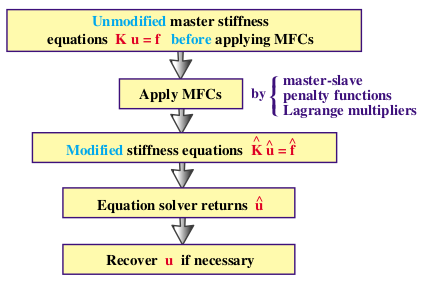
\includegraphics[width=0.70\textwidth]{img/mfc_schematic.png}
    \caption{Schematics of MFC application.}
    \label{fig:MFC-schematic}
\end{figure}


\section{Methods for Imposing MFCs}

Accounting for MFCs is done, at least conceptually, by changing the assembled master
stiffness equations to produce a \textit{modified} system of equations:

\begin{equation}\label{mfc-modification}
    \m{K} \m{u} = \m{f} \overset{MFC}{\implies}
    \hat{\m{K}} \hat{\m{u}} = \hat{\m{f}}
\end{equation}

The modification process \eqref{mfc-modification} is also called  \textit{constraint}
\textit{application} or \textit{constraint imposition}. The modified system
is that submitted to the equation solver, which returns $ \hat{\m{u}} $.

Three methods for applying \textbf{MFCs} are written below:

\begin{enumerate}
    \item \textit{Master-Slave Elimination}

        The DOFs involved in each MFC are separated into master and slave freedoms.
        The slave freedoms are then explicitely eliminated. The modified equations
        do not contain the slave freedoms.

    \item \textit{Penalty Augmentation}

        Also called the \textit{penalty function method}. Each \textbf{MFC}
        is viewed as the presence of a fictious elastic structural element called
        the \textit{penalty element} that enforces it approximately. This element
        is parametrized by a numerical \textit{weight}. The exact constraint is
        recovered if the weight goes to \textbf{infinity}. The MFCs are imposed
        by augmenting the finite element model with the penalty elements.

    \item \textit{Lagrange Multiplier Adjunction}

        For each MFC an additional unknown is adjoined to the master stiffness
        equations. Physically this set of unknowns represent
        \textit{constraint forces} that would enforce the constraints exactly
        should they be applied to the unconstrained system.
\end{enumerate}

The master stiffness equations are assembled ignoring all constraints. Then the MFCs
are imposed by appropriate modification of those equations. There are, however,
two important practical differences:

\begin{enumerate}
    \item The modification process is not unique because there are alternative
        constraint imposition methods. These methods offer tradeofss in generality,
        programming implementation complexity, computational effort, numerical
        accuracy and stability.

    \item In the implementation of some of these methods - notably penalty augmentation
        - constraint imposition and assembly are carried out simultaneously. In that
        case the framework "first assemble, then modify", is not strictly respected
        in the actual implementation.
\end{enumerate}


\subsection{MFC Matrix Forms}

Matrix forms of \textit{linear} \textbf{MFCs} are often convenient for compact
notation. An individual constraint may be written:

\begin{equation}\label{mfc-matrix}
    \begin{bmatrix}
        1 & -2 & 1
    \end{bmatrix}
    \begin{bmatrix}
        u_{x2} \\
        u_{x4} \\
        u_{x6}
    \end{bmatrix}
    = 0.25
\end{equation}

In direct matrix notation:

\begin{equation}\label{mfc-direct}
    \closure{\m{a}}_i \closure{\m{u}}_i = g_i, \quad (no\ sum\ on\ i)
\end{equation}

in which index $ i\ (i = 1, 2,\dots) $ identifies constraint, $ \closure{\m{a}}_i $
is a row vector, $ \closure{\m{u}}_i $ collects the set of \textbf{DOFs}
that participate in the constraint, and $ g_i $ is the \textbf{RHS} scalar.
The bars over $ \m{a} $ and $ \m{u} $ distinguishes
\eqref{mfc-direct} from the expanded form below.

\begin{figure}[ht]
    \centering
    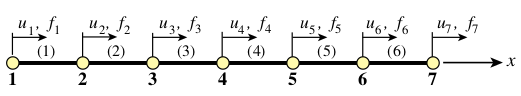
\includegraphics[width=0.70\textwidth]{img/1D_mfc_bar.png}
    \caption{1D problem discretized with six bar finite elements.}
    \label{fig:1D-MFC-bar-png}
\end{figure}

For method description and general proof it is often convenient to \textit{expand}
matrix forms so that they embody \textit{all} DOFs. For example, if
\eqref{mfc-matrix} is a part of a two-dimensional FE model with 12 DOFs:

$ u_{x1}, u_{y1}, \dots, u_{y6} $, the LHS row vector may be expanded with
9 zeros as follows:

\begin{equation}
    \begin{bmatrix}
        0 & 0 & 1 & 0 & 0 & 0 & -2 & 0 & 0 & 0 & 1 & 0
    \end{bmatrix}
    \begin{bmatrix}
        u_{x1} \\
        u_{y1} \\
        u_{x2} \\
        \vdots \\
        u_{y6}
    \end{bmatrix}
    = 0.25
\end{equation}

In which case the matrix notation:

\begin{equation}\label{mfc-expanded}
    \m{a}_i \m{u}_i = g_i
\end{equation}

is used. Finally, all \textbf{MFCs} expressed as \eqref{mfc-expanded} may be collected
into a single matrix relation:

\begin{equation}\label{mfc-expanded-matrix}
    \m{A} \m{u} = \m{g}
\end{equation}

in which the rectangular matrix $ \m{A} $ is formed by stacking the
$ \m{a}_i $'s as rows and column vector $ \m{g} $ is formed by stacking
the $ g_i $s as entries. If there are 12 DOFs in $ \m{u} $ and \textbf{5 MFCs},
then $ \m{A} $ will be $ 5 \times 12 $.


\subsection{The Example Structure}

The one-dimensional FE discretization shown in Figure \ref{fig:1D-MFC-bar-png}
will be used to illustrate the three \textbf{MFC} application methods. The
strucuture consists of six bar elements connected by seven nodes that can only
displace in the \textit{x} direction.

Before imposing various \textbf{multifreedom} constraints discussed below, the master
stiffness equations for this problem are assumed to be:

\begin{equation}\label{master-stiffness-6-bar}
    \begin{bmatrix}
        K_{11} & K_{12} & 0 & 0 & 0 & 0 & 0 \\
        K_{12} & K_{22} & K_{23} & 0 & 0 & 0 & 0 \\
        0 & K_{23} & K_{33} & K_{34} & 0 & 0 & 0 \\
        0 & 0 & K_{34} & K_{44} & K_{45} & 0 & 0 \\
        0 & 0 & 0 & K_{45} & K_{55} & K_{56} & 0 \\
        0 & 0 & 0 & 0 & K_{56} & K_{66} & K_{67} \\
        0 & 0 & 0 & 0 & 0 & K_{67} & K_{77}
    \end{bmatrix}
    \begin{bmatrix}
        u_1 \\
        u_2 \\
        u_3 \\
        u_4 \\
        u_5 \\
        u_6 \\
        u_7
    \end{bmatrix}
    = \begin{bmatrix}
        f_1 \\
        f_2 \\
        f_3 \\
        f_4 \\
        f_5 \\
        f_6 \\
        f_7
    \end{bmatrix}
\end{equation}

or

\begin{equation}\label{mfc-ms-master-equation}
    \m{K} \m{u} = \m{f}
\end{equation}

The nonzero stifness coefficients $ K_{ij} $ in \eqref{master-stiffness-6-bar}
depend on the bar rigidity properties. For example, if
$ E^e A^e / L^e = 100 $ for each element $ e = 1, \dots , 6 $, then
$ K_{11} = K_{77} = 100 $, $ K_{22} = \dots = K_{66} = 200 $,
$ K_{12} = K_{23} = \dots = K_{67} = -100 $. However, for the purposes of the
following treatment the coefficient may be kept arbitrary. The component index
$ x $ in the nodal displacements $ u $ and nodal forces $ f $ has been omitted
for brevity.

Now let us specify a \textbf{MFC} that states that nodes \textbf{2} and \textbf{6}
must move by the same amount:

\begin{equation}\label{mfc-2-6}
    u_2 = u_6
\end{equation}

Passing all node displacements to the RHS gives the canonical form:

\begin{equation}\label{mcf-canonical-2-6}
    u_2 - u_6 = 0
\end{equation}

Constraint conditions of this type are sometimes called \textbf{rigid links}
because they can be mechanically interpreted as forcing node points 2 and 6
to move together as if they were tied tohether by a rigid member.

We now study the imposition of constraint \eqref{mcf-canonical-2-6} on the master equations
\eqref{master-stiffness-6-bar} by the methods mentioned above. First the master-slabe
method is treated

\section{The Master-Slave Method}

To apply this method by \textit{hand}, the MFCs are taken one at a time. For each
constraint a \textbf{slave} DOF is chosen. The freedoms remaining in that constraint
are labeled \textbf{master}. A new set of DOFs $ \m{\hat{u}} $ is established
by removing all slave freedoms from $ \m{u} $. This new vector contains
master freedoms as well as those that do not appear in the MFCs. A matrix transformation
equation that relates $ \m{u} $ to $ \m{\hat{u}} $ is generated. This
equation is used ot apply a congruent transformation to the master stiffness equations.
This procedure yields a set of modified stiffness equations that are expressed in terms
of the new freedom set $ \m{\hat{u}} $. Because the modified system does not contain
the slave freedoms, these have been effectively eliminated.

\subsection{A One-Constraint Example}

The mechanics if the process is best seen by going through an example. To impose
\eqref{mcf-canonical-2-6} pick $ u_6 $ as slave and $ u_2 $ as master. Relate the
original unknowns $ u_1, \dots, u_7 $ to the new set in which $ u_6 $ is missing:

\begin{equation}\label{mfc-ms-transformation}
    \begin{bmatrix}
        u_1 \\
        u_2 \\
        u_3 \\
        u_4 \\
        u_5 \\
        u_6 \\
        u_7
    \end{bmatrix}
    = \begin{bmatrix}
        1 & 0 & 0 & 0 & 0 & 0 \\
        0 & 1 & 0 & 0 & 0 & 0 \\
        0 & 0 & 1 & 0 & 0 & 0 \\
        0 & 0 & 0 & 1 & 0 & 0 \\
        0 & 1 & 0 & 0 & 0 & 0 \\
        0 & 0 & 0 & 0 & 0 & 1
    \end{bmatrix}
    \begin{bmatrix}
        u_1 \\
        u_2 \\
        u_3 \\
        u_4 \\
        u_5 \\
        u_7
    \end{bmatrix}
\end{equation}

This is the required transformation relation. In compact form:

\begin{equation}
    \m{u} = \m{T} \m{\hat{u}}
\end{equation}


Replacing \eqref{mfc-ms-transformation} into \eqref{mfc-ms-master-equation} and
premultiplying by $ \m{T}^T $ yields the modified system:

\begin{equation}\label{mfc-ms-modified-system}
    \m{\hat{K}} \m{\hat{u}} = \m{\hat{f}}, \quad
    in\ which \quad \m{\hat{K}} = \m{T}^T \m{K} \m{T}, \quad
    \m{\hat{f}} = \m{T}^T \m{f}.
\end{equation}

\begin{bbox}
    The form of modified system \eqref{mfc-ms-modified-system} can be remembered
    by a simple mnemonic rule: premultiply both sides of $
    \m{T} \m{\hat{u}} = \m{u} $
    by $ \m{T}^T \m{K} $ and replace $ \m{K} \m{u} $ by
    $ \m{f} $ on the right hand side.
\end{bbox}

Carrying out the indicated matrix multiplication yields:

\begin{equation}\label{mfc-ms-modified-master}
    \begin{bmatrix}
        K_{11} & K_{12} & 0 & 0 & 0 & 0 \\
        K_{12} & K_{22} + K_{66} & K_{23} & 0 & K_{56} & K_{67} \\
        0 & K_{23} & K_{33} & K_{34} & 0 & 0 \\
        0 & 0 & K_{34} & K_{44} & K_{45} & 0 \\
        0 & K_{56} & 0 & K_{45} & K_{55} & 0 \\
        0 & K_{67} & 0 & 0 & 0 & K_{77}
    \end{bmatrix}
    \begin{bmatrix}
        u_1 \\
        u_2 \\
        u_3 \\
        u_4 \\
        u_5 \\
        u_7
    \end{bmatrix}
    = \begin{bmatrix}
        f_1 \\
        f_2 + f_6 \\
        f_3 \\
        f_4 \\
        f_5 \\
        f_7
    \end{bmatrix}
\end{equation}

Equation \eqref{mfc-ms-modified-master} is a new linear system containing 6 equations
in the remaining 6 unknowns $ u_1, u_2, u_3, u_4, u_5\ and\ u_7 $. Upon
solving it, $ u_6 $ is recovered from the constraint \eqref{mfc-2-6}.

\begin{bbox}
    For a simple freedom constraint such as $ u_4 = 0 $ the only possible choice of slave
    is of course $ u_4 $ and there is no master. The congruent transformation is then
    nothing more than the elimination of $ u_4 $ by striking out rows and columns from
    the master stiffness equations.
\end{bbox}


\subsection{Multiple Homogeneous MFCs}

The matrix equation \eqref{mfc-ms-modified-system} in fact holds for the general
case of multiple homogeneous linear constraints. Direct establishment of the transformation
equation, however, is more complicated if slave freedoms in one constraint appear as masters
in another. To illustrate this point, suppose that for the example system we have three
homogeneous MFCs:

\begin{eqarray}\label{mfc-ms-3-constraints}
    u_2 - u_6 &= 0 \\
    u_1 + 4 u_4 &= 0 \\
    2 u_3 + u_4 + u_5 &= 0
\end{eqarray}

Picking as slave freedoms $ u_6 $, $ u_4 $ and $ u_3 $ from the first, second and third
constraint, respectively, we can solve for them as:

\begin{eqarray}
    u_6 &= u_2 \\
    u_4 &= -\frac{1}{4} u_1 \\
    u_3 &= -\frac{1}{2} \left( u_4 + u_5 \right) = \frac{1}{8} u_1 - \frac{1}{2} u_5
\end{eqarray}

Observe that solving for $ u_3 $ from the third constraint brings $ u_4 $ to the RHS.
But because $ u_4 $ is also slave freedom (it was chosen as such for the second constraint)
it is replaced in favor of $ u_1 $ using $ u_4 = -\frac{1}{4} u_1 $. The matrix form
transformation is:

\begin{equation}\label{mfc-ms-multiple-freedoms}
    \begin{bmatrix}
        u_1 \\
        u_2 \\
        u_3 \\
        u_4 \\
        u_5 \\
        u_6 \\
        u_7
    \end{bmatrix}
    = \begin{bmatrix}
        1 & 0 & 0 & 0 \\
        0 & 1 & 0 & 0 \\
        \frac{1}{8} & 0 & -\frac{1}{2} & 0 \\
        -\frac{1}{4} & 0 & 0 & 0 \\
        0 & 0 & 1 & 0 \\
        0 & 1 & 0 & 0 \\
        0 & 0 & 0 & 1
    \end{bmatrix}
    \begin{bmatrix}
        u_1 \\
        u_2 \\
        u_5 \\
        u_7
    \end{bmatrix}
\end{equation}

The modified master system is now formed through the congruent
transformation \eqref{mfc-ms-modified-system}.
Note that the slave freedoms selected from each
constraint must be distinct. For example the choice $ u_6 $, $ u_4 $ and $ u_4 $
would be inadmissible as long the constraints are independent. This rule is easy
to enforce when slave freedoms are chosen by hand, but can lead to implementation
and numerical difficulties when it is programmed as an automated procedure, as
further discussed later.

\begin{bbox}
    The 3 MFCs \eqref{mfc-ms-3-constraints} with $ u_6 $, $ u_4 $ and $ u_2 $ chosen
    as slaves and $ u_1 $, $ u_2 $ and $ u_5 $ chosen as masters, may be presented
    in the partitioned matrix form:

    \begin{equation}
        \begin{bmatrix}
            0 & 0 & 1 \\
            0 & 4 & 0 \\
            2 & 1 & 0
        \end{bmatrix}
        \begin{bmatrix}
            u_3 \\
            u_4 \\
            u_6
        \end{bmatrix}
        = \begin{bmatrix}
            0 & 1 & 0 \\
            -1 & 0 & 0 \\
            0 & 0 & -1
        \end{bmatrix}
        \begin{bmatrix}
            u_1 \\
            u_2 \\
            u_5
        \end{bmatrix}
    \end{equation}

     This may be compactly written as:

     \begin{equation}
         \m{A}_s \m{u}_s + \m{A}_m \m{u}_m = \m{0}
     \end{equation}

     Solving for the slave freedoms gives

     \begin{equation}
         \m{u}_s = -\m{A}_s^{-1} \m{A}_m \m{u}_m
     \end{equation}

     Expanding with zeros to fill out $ \m{u} $ and $ \m{\hat{u}} $
     produces \eqref{mfc-ms-multiple-freedoms}. Note that non-singularity of
     $ \m{A}_s $ is essential for this method to work.
\end{bbox}


\subsection{Nonhomoheneous MFCs}

Extension to nonhomogeneous constraints is immediate. In this case the transformation
equation becomes nonhomogeneous. For example suppose that \eqref{mcf-canonical-2-6}
has non-zero prescribed value:

\begin{equation}\label{mcf-canonical-2-6-nonhomogeneous}
    u_2 - u_6 = 0.2
\end{equation}

Nonzero RHS values such as $ 0.2 $ in \eqref{mcf-canonical-2-6-nonhomogeneous}
may often be interpreted physically as "gaps" (thus the use of the symbol
$ \m{g} $ in the matrix form). Chose $ u_6 $ again as slave: $ u_6 = u_2 - 0.2 $
and build the transformation:

\begin{equation}
    \begin{bmatrix}
        u_1 \\
        u_2 \\
        u_3 \\
        u_4 \\
        u_5 \\
        u_6 \\
        u_7
    \end{bmatrix}
    = \begin{bmatrix}
        1 & 0 & 0 & 0 & 0 & 0 \\
        0 & 1 & 0 & 0 & 0 & 0 \\
        0 & 0 & 1 & 0 & 0 & 0 \\
        0 & 0 & 0 & 1 & 0 & 0 \\
        0 & 0 & 0 & 0 & 1 & 0 \\
        0 & 1 & 0 & 0 & 0 & 0 \\
        0 & 0 & 0 & 0 & 0 & 1
    \end{bmatrix}
    \begin{bmatrix}
        u_1 \\
        u_2 \\
        u_3 \\
        u_4 \\
        u_5 \\
        u_7
    \end{bmatrix} +
    \begin{bmatrix}
        0 \\
        0 \\
        0 \\
        0 \\
        0 \\
        -0.2 \\
        0
    \end{bmatrix}
\end{equation}

In the compact matrix form:

\begin{equation}\label{mfc-ms-gap}
    \m{u} = \m{T} \m{\hat{u}} + \m{g}
\end{equation}

Here the constraint gap vector $ \m{g} $ is nonzero and $ \m{T} $ is the same
as before. To get the modified system applying the shortcut rule, premultiply
both sides of \eqref{mfc-ms-gap} by $ \m{T}^T \m{K} $, replace
$ \m{K} \m{u} $ by $ \m{f} $ and pass the data to the RHS:

\begin{equation}\label{mfc-ms-modified-system-gap}
    \m{\hat{K}} \m{\hat{u}} = \m{\hat{f}}, \quad
    in\ which \quad \m{\hat{K}} = \m{T}^T \m{K} \m{T}, \quad
    \m{\hat{f}} = \m{T}^T \left( \m{f} -\m{K} \m{g} \right).
\end{equation}

Upon solving \eqref{mfc-ms-modified-system-gap} for $ \m{\hat{u}} $, the
complete displacement vector is recovered from \eqref{mfc-ms-gap}. For the MFC
\eqref{mcf-canonical-2-6-nonhomogeneous} this technique gives the system:

\begin{equation}
    \begin{bmatrix}
        K_{11} & K_{12} & 0 & 0 & 0 & 0 \\
        K_{12} & K_{22} + K_{66} & K_{23} & 0 & K_{56} & K_{67} \\
        0 & K_{23} & K_{33} & K_{34} & 0 & 0 \\
        0 & 0 & K_{34} & K_{44} & K_{45} & 0 \\
        0 & K_{56} & 0 & K_{45} & K_{55} & 0 \\
        0 & K_{67} & 0 & 0 & 0 & K_{77}
    \end{bmatrix}
    \begin{bmatrix}
        u_1 \\
        u_2 \\
        u_3 \\
        u_4 \\
        u_5 \\
        u_7
    \end{bmatrix}
    = \begin{bmatrix}
        f_1 \\
        f_2 + f_6 - 0.2 K_{66} \\
        f_3 \\
        f_4 \\
        f_5 - 0.2 K_{56} \\
        f_7 - 0.2 K_{67}
    \end{bmatrix}
\end{equation}


\subsection{The General Case}

For implementation in general-purpose programs the \textbf{master-slave method}
can be described as follows. The \textbf{DOFs} in $ \m{u} $ are classified
into three types: \textbf{independent} or unconstrained, \textbf{masters} and
\textbf{slaves}. The unconstrained DOFs are those that do not appear in any MFC.
Label these sets as $ \m{u}_u $, $ \m{u}_m $ and $ \m{u}_s $,
respectively, and partition the stiffness equations accordingly:

\begin{equation}\label{mfc-ms-partitioned}
    \begin{bmatrix}
        \m{K}_{uu} & \m{K}_{um} & \m{K}_{us} \\
        \m{K}_{um}^T & \m{K}_{mm} & \m{K}_{ms} \\
        \m{K}_{us}^T & \m{K}_{ms}^T & \m{K}_{ss}
    \end{bmatrix}
    \begin{bmatrix}
        \m{u}_u \\
        \m{u}_m \\
        \m{u}_s
    \end{bmatrix}
    = \begin{bmatrix}
        \m{f}_u \\
        \m{f}_m \\
        \m{f}_s \\
    \end{bmatrix}
\end{equation}

The MFCs may be written in matrix form as:

\begin{equation}
    \m{A}_m \m{u}_m + \m{A}_s \m{u}_s = \m{g}_A
\end{equation}

where $ \m{A}_s $ is assumed square and nonsingular. If so we can solve for
the slave freedoms:

\begin{equation}
    \m{u}_s = \m{A}_s^{-1} \m{A}_m \m{u}_m
    + \m{A}_s^{-1} \m{g}_A
    \eqd \m{T} \m{u}_m + \m{g}
\end{equation}

where $ \eqd $ means \textit{equal by definition}. Inserting into the partitioned
sitffness equation \eqref{mfc-ms-partitioned} and symmetrizing yields:

\begin{equation}
    \begin{bmatrix}
        \m{K}_{uu} & \m{\hat{K}}_{um} \\
        \m{\hat{K}}_{um}^T &
        \m{\hat{K}}_{mm}
    \end{bmatrix}
    \begin{bmatrix}
        \m{u}_u \\
        \m{u}_m
    \end{bmatrix}
    = \begin{bmatrix}
        \m{f}_u - \m{K}_{us} \m{g} \\
        \m{f}_m - \m{K}_{ms} \m{g}
    \end{bmatrix}
\end{equation}

where $ \m{\hat{K}}_{um} = \m{K}_{um} + \m{K}_{us} \m{T} $ \\
and $ \m{\hat{K}}_{mm} = \m{K}_{mm} + \m{T}^T \m{K}_{ms}^T
+ \m{K}_{ms} \m{T} + \m{T}^T \m{K}_{ss} \m{T} $.

It is seen that the misleading simplicity of the handworked example is gone.


\subsection{Retaining the Original Freedoms}

A potential disadvantage of the master-slave methid in computer work is that it
requires a rearrangement of the original stiffness equations because
$ \m{\hat{u}} $ is a subset of $ \m{u} $. The disadvantage can be
annoying when sparse matrxi storage schemes are used for the stiffness matrix,
and becomes intolerable if secondary storage is used for that purpose.

With a bit of trickery it is possible to maintain the original freedom ordering.
Let us display it for the example problem under \eqref{mcf-canonical-2-6}.
Instead of \eqref{mfc-ms-transformation}, use the \textit{square} transformation:

\begin{equation}
    \begin{bmatrix}
        u_1 \\
        u_2 \\
        u_3 \\
        u_4 \\
        u_5 \\
        u_6 \\
        u_7
    \end{bmatrix}
    = \begin{bmatrix}
        1 & 0 & 0 & 0 & 0 & 0 & 0 \\
        0 & 1 & 0 & 0 & 0 & 0 & 0 \\
        0 & 0 & 1 & 0 & 0 & 0 & 0 \\
        0 & 0 & 0 & 1 & 0 & 0 & 0 \\
        0 & 0 & 0 & 0 & 1 & 0 & 0 \\
        0 & 1 & 0 & 0 & 0 & 0 & 0 \\
        0 & 0 & 0 & 0 & 0 & 0 & 1
    \end{bmatrix}
    \begin{bmatrix}
        u_1 \\
        u_2 \\
        u_3 \\
        u_4 \\
        u_5 \\
        \overline{u}_6 \\
        u_7
    \end{bmatrix}
\end{equation}

in which $ \overline{u}_6 $ is a \textit{placeholder} for the slave freedom $ u_6 $.
The modified equations are:

\begin{equation}
    \begin{bmatrix}
        K_{11} & K_{12} & 0 & 0 & 0 & 0 & 0 & 0 \\
        K_{12} & K_{22} + K_{66} & K_{23} & 0 & 0 & K_{56} & 0 & K_{67} \\
        0 & K_{23} & K_{33} & K_{34} & 0 & 0 & 0 & 0 \\
        0 & 0 & K_{34} & K_{44} & K_{45} & 0 & 0 & 0 \\
        0 & K_{56} & 0 & K_{45} & K_{55} & 0 & 0 & 0 \\
        0 & K_{67} & 0 & 0 & 0 & 0 & 0 & K_{77}
    \end{bmatrix}
    \begin{bmatrix}
        u_1 \\
        u_2 \\
        u_3 \\
        u_4 \\
        u_5 \\
        \overline{u}_6 \\
        u_7
    \end{bmatrix}
    = \begin{bmatrix}
        f_1 \\
        f_2 + f_6 \\
        f_3 \\
        f_4 \\
        f_5 \\
        0 \\
        f_7
    \end{bmatrix}
\end{equation}

which are submitted to the equation solver. If the solver is not trained to skip
zero rows and columns, a one should be placed in the diagonal entry for the
$ \overline{u}_6 $ equation. The solver will return $ \overline{u}_6 = 0 $,
and this placeholder value is replaced by $ u_2 $.


\subsection{Model Reduction by Kinematic Constraints}

The congruent transformation equations \eqref{mfc-ms-modified-system}
and \eqref{mfc-ms-modified-system-gap} have additional applications beyond the
master-slave method. An important one is \textit{model reduction by kinematic constraints}.
Trough this procedure the number of \textbf{DOFs} of a static or dynamic FEM model
is reduced by a significant number, typycally to $ 1 \% - 10 \% $ of the original number.
This is done by taking a lot of slaves and a few masters. Only the masters are left
after the transformation. The reduced model is commonly used in subsequent calculations
as a component of a larger system, particularly during design or in parameter
identification.


\textbf{Example:}

\begin{figure}[ht]
    \centering
    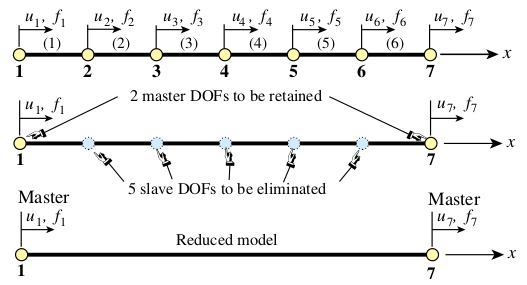
\includegraphics[width=0.90\textwidth]{img/mfc_model_reduction_end.png}
    \caption{Model reduction of the example structure to the end freedoms}
    \label{fig:mfc-model-reduction-end-png}
\end{figure}

Consider the bar assembly of Figure \ref{fig:mfc-model-reduction-end-png}.
Assume that the only masters are the end motions $ u_1 $ and $ u_7 $, as
illustrated in Figure \ref{fig:mfc-model-reduction-end-png}, and interpolate
all freedoms linearly:

\begin{equation}
    \begin{bmatrix}
        u_1 \\
        u_2 \\
        u_3 \\
        u_4 \\
        u_5 \\
        u_6 \\
        u_7
    \end{bmatrix}
    = \begin{bmatrix}
        1 & 0 \\
        \frac{5}{6} & \frac{1}{6} \\
        \frac{4}{6} & \frac{2}{6} \\
        \frac{3}{6} & \frac{3}{6} \\
        \frac{2}{6} & \frac{4}{6} \\
        \frac{1}{6} & \frac{5}{6} \\
        0 & 1 \\
    \end{bmatrix}
    \begin{bmatrix}
        u_1 \\
        u_7
    \end{bmatrix}, \quad or \quad
    \m{u} = \m{T} \m{\hat{u}}
\end{equation}

The reduced-order-model (\textbf{ROM}) equations are:

\begin{equation}
    \m{\hat{k}} \m{\hat{u}}
    = \m{T}^T \m{K} \m{T} \m{\hat{u}}
    = \m{T}^T \m{f}
    = \m{\hat{f}}
\end{equation}

or in detail

\begin{equation}
    \begin{bmatrix}
        \hat{K}_{11} & \hat{K}_{17} \\
        \hat{K}_{17}^T & \hat{K}_{77}
    \end{bmatrix}
    \begin{bmatrix}
        u_1 \\
        u_7
    \end{bmatrix}
    = \begin{bmatrix}
        \hat{f}_1 \\
        \hat{f}_7
    \end{bmatrix}
\end{equation}

in which:

\begin{eqarray}
    \hat{K}_{11} &= \frac{1}{36}
    \left( 36 K_{11} + 60 K_{12} + 25 K_{22} + 40 K_{23} + 16 K_{33} + 24 K_{34} \right. \\
                 &+  \left. 9 K_{44} + 12 K_{45} + 4 K_{55} + 4 K_{56} + K_{66} \right) \\
    \hat{K}_{17} &= \frac{1}{36}
    \left( 6 K_{12} + 5 K_{22} + 14 K_{23} + 8 K_{33} + 18 K_{34} + 9 K_{44} \right. \\
                 &+ \left. 18 K_{45} + 8 K_{55} + 14 K_{56} + 5 K_{66} + 6 K_{67} \right) \\
    \hat{K}_{77} &= \frac{1}{36}
    \left( K_{22} + 4 K_{23} + 4 K_{33} + 12 K_{34} + 9 K_{44} + 24 K_{45} \right. \\
                 &+ \left. 16 K_{55} + 40 K_{56} + 25 K_{66} + 60 K_{67} + 36 K_{77} \right) \\
    \hat{f}_1 & = \frac{1}{6}
    \left(
        6 f_1 + 5 f_2 + 4 f_3 + 3 f_4 + 2 f_5 + f_6
    \right) \\
    \hat{f}_7 & = \frac{1}{6}
    \left(
        f_2 + 2 f_3 + 3 f_4 + 4 f_5 + 5 f_6 + 6 f_7
    \right) \\
\end{eqarray}

This reduces the order of the FEM model from 7 to 2. The \textbf{key feature} is that
the masters are picked \textbf{a priori}, as the freedoms to be retained in the
model for further use.

\begin{bbox}
    Model reduction can be also done by the \textbf{static condensation} (Guyan)
    method. As its name indicates, condensation is restricted to static analysis.
    On the other hand, for such problems it is exact whereas model reduction by
    kinematic constraints generally introduces approximations.
\end{bbox}


\subsection{Assesment of the Master-Slave Method}

The \textbf{Master-Slave Method} enjoys the advantage of being \textbf{exact}
(except for inevitable solution errors from finite number precision) and of
reducing the nuber of unknowns. The concept is also easy to explain and learn.
The main implementation drawback is the complexity of the general case.
The complexity is due to three factors:

\begin{enumerate}
    \item The equations may have to be rearranged because of the disappearance
        of the slave freedoms. This drawback can be alleviated, however,
        by the \textbf{placeholder} trick.

    \item An auxiliary linear system has to be assembled and solved to produce
        the transformation matrix $ \m{T} $ and vector $ \m{g} $.

    \item The transformation process may generate many additional matrix terms.
        If a sparse matrix storage scheme is used for $ \m{K} $, the logic
        for allocating memory and storing these entries can be difficult
        and expensive.
\end{enumerate}

The level of complexity depends on the generality allowed as well as on programming
decisions. If $ \m{K} $  is stored as full matrix and slave freedom coupling in
the MFCs is disallowed the logic is simple (this is the case in model reduction,
since each slave freedom appears in one and only one MFC). On the other hand,
if arbitrary couplings are permitted and $ \m{K} $ is placed in secondary
(disk) storage according to some sparse scheme, the complexity can become
overwhelming.

Another, more subtle, drawback of this method is that it requires decisions as to
which DOFs are to be treated as slaves. This can lead to implementation and numerical
stability problems. Although for disjointed constraints the process can be programmed
in reliable form, in more general cases of coupled constraint equations it can
lead to incorrect decisions. For example, suppose that in the example problem
you have the following two MFCs:

\begin{eqarray}
    \frac{1}{6} u_2 + \frac{1}{2} u_4 &= u_6 \\
    u_3 + 6 u_6 &= u_7
\end{eqarray}

For numerical stability reasons it is usually better to pick as slaves the freedoms
with largest coefficients. If this is done, the program would select $ u_6 $ as
slave freedoms from both constraints. This leads to a contradiction because
having two constraints we must eliminate two slave DOFs, not just one. The resulting
modified system would in fact be inconsistent. Although this defect can be easily fixed
by the program logic in this case, one can imagine the complexity burden if faced
with hundreds of thousands of MFCs.

Serious numerical problems can arise if the MFCs are not independent. For example:

\begin{eqarray}
    \frac{1}{6} u_2 &= u_6 \\
    \frac{1}{3} u_3 + 6 u_6 &= u_7 \\
    u_2 + u_3 - u_7 &= 0
\end{eqarray}

The last constraint is an exact linear combination of the first two. If the program
blindly choses $ u_2 $, $ u_3 $ and $ u_7 $ as slaves, the modified system is
incorrect because we eliminate three equations when in fact there are only two
independent constraints. Exact linear dependence, as before, can be recognised by
a rank analysis of the $ \m{A}_s $ matrix defined. In the floating-point
arithmetic, however, such detection may fail because that kind of computation is
inexact bt nature (The safest technique to identify dependencies is to do
a singular value decomposition (SVD) of $ \m{A}_s $. This can be, however,
prohibitively expensive if one is dealing with hundreds of thousands of constraints.).

The complexithy of slave selection is in fact equivalent to that of automatically
selecting kinematic redundancies in the Force Method of structural analysis.
\textbf{It has led implementators of programs that use this method to require masters}
\textbf{and slaves to be prescribed in the input data, thus transfering the burden}
\textbf{to users}.

The method is not generally extensible to nonlinear constraints without case
by case programming.

In conclusion, the master-slave method is useful when a few simple linear constraints
are imposed by hand. As a general purpose technique for FEM it suffers from
complexity and lack of robustness. It is worth learning, however, because of the
great importance of congruent transformations in
\textit{model reduction} for static and dynamic problems.

\subsubsection{Bibliograpy}

Felippa - IFEM (Chapter 8)

Zienkiewicz and Taylor - The Finite Element Method \textit{4th ed.} 1988


\section{The Penalty Method}

\begin{figure}[ht]
    \centering
    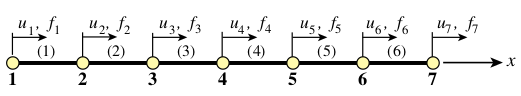
\includegraphics[width=0.70\textwidth]{img/1D_mfc_bar.png}
    \caption{1D problem discretized with six bar finite elements.}
    \label{fig:1D-MFC-bar-png-2}
\end{figure}

The penalty method will be first presented using a physical interpretation,
leaving the mathematical formulation to a subsequent section. Constider again
the bar example structure. To impose $ u_2 = u_6 $ imagine that nodes 2 and 6
are connected with a "fat" bar of axial stiffness $ w $, labeled with element
number 7, as shown in Figure \ref{fig:1D-MFC-bar-penalty-png}. This bar is called \textbf{penalty element} and
$ w $ is its \textbf{penalty weight}.

\begin{figure}[ht]
    \centering
    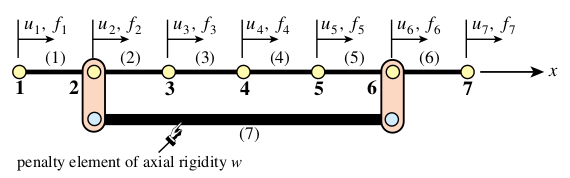
\includegraphics[width=0.70\textwidth]{img/1D_mfc_bar_penalty.png}
    \caption{Adjusnction of a fictious penalty bar of axial stiffness $ w $,
    identified as element 7, to enforce $ u_2 = u_6 $.}
    \label{fig:1D-MFC-bar-penalty-png}
\end{figure}

Such an element, albeit fictious, can be treated exactly like another bar element
insofar as continuing the assembly of the master stiffness equations. The penalty
element stiffness equations $ \m{K}^{(7)} \m{u}^{(7)} = \m{f}^{(7)} $,
are:

\begin{equation}
    w \begin{bmatrix}
        \phantom{-}1 & -1 \\
        -1 & \phantom{-}1
    \end{bmatrix}
    \begin{bmatrix}
        u_2 \\
        u_6
    \end{bmatrix}
    = \begin{bmatrix}
        f_2^{(7)} \\
        f_6^{(7)}
    \end{bmatrix}
\end{equation}

Because there is one freedom per node, the two local element freedoms map into global
freedoms 2 and 6, respectively. Using the assembly rules we obtain the following
modified master stiffness equations: $ \m{\hat{K}} \m{\hat{u}} = \m{\hat{f}} $,
which shown in detail are:

\begin{equation}\label{mfc-penalty-master-stiffnes}
    \begin{bmatrix}
        K_{11} & K_{12} & 0 & 0 & 0 & 0 & 0 \\
        K_{12} & K_{22} + w & K_{23} & 0 & 0 & -w & 0 \\
        0 & K_{23} & K_{33} & K_{34} & 0 & 0 & 0 \\
        0 & 0 & K_{34} & K_{44} & K_{45} & 0 & 0 \\
        0 & 0 & 0 & K_{45} & K_{55} & K_{56} & 0 \\
        0 & -w & 0 & 0 & K_{56} & K_{66} + w & K_{67} \\
        0 & 0 & 0 & 0 & 0 & K_{67} & K_{77}
    \end{bmatrix}
    \begin{bmatrix}
        u_1 \\
        u_2 \\
        u_3 \\
        u_4 \\
        u_5 \\
        u_6 \\
        u_7
    \end{bmatrix}
    = \begin{bmatrix}
        f_1 \\
        f_2 \\
        f_3 \\
        f_4 \\
        f_5 \\
        f_6 \\
        f_7
    \end{bmatrix}
\end{equation}

This system can now be submitted to the equation solver. Note that
$ \m{\hat{u}} \equiv \m{u} $ and only $ \m{K} $ has changed.

\subsection{Choosing the Penalty Weight}

What happens when \eqref{mfc-penalty-master-stiffnes} is solved numerically?
If a \textit{finite} weight $ w $ is chosen the constraint $ u_2 = u_6 $ is
approximately satisfied in the sense that one gets $ u_2 - u_6 = e_g $, where
$ e_g \neq 0 $. The "gap error" $ e_g $ is called the \textit{constraint violation}.
The magnitude $ \left| e_g \right| $ of this violation depends on the wight:
the larger $ w $, the smaller the violation. More precisely, it can be shown
that $ | e_g | $ becomes ptoportional to $ \frac{1}{w} $ as $ w $ gets to be
sufficiently large. For example, raising $ w $ from, say, $ 10^6 $ to $ 10^7 $
can be expected to cut the constraint violation roughly by $ 10 $ if the physical
stiffnesses are smalle compared to $ w $.

Therefore it seems as if the proper strategy should be: try to make $ w $ as large
as possible while respecting the computer overflow limits. However, this is misleading.
As the penalty weight $ w $ tends to $ \infty $ the modified stiffness matrix becomes
more and more \textit{ill-conditioned with respect to inversion}.

To make this point clear, suppose for definiteness that rigidites
$ E^e A^e / L^e $ of the actual bars $ e = 1, \dots, 6 $ are unity, that
$ w >> 1 $, and that the computer solving the stiffness equations has a
floating-point precision of 16 decimal places. Numerical analusts characterize such
precision by sayinf that $ \epsilon_f = \mathcal{O}(10^{-16}) $, where
$ | \epsilon_f | $ is the smallest power of 10 that perceptibly adds to 1 in
floating-point arithmetic (this is usually done not for decimal numbers but
base-2 binary numbers). The modified stiffness matrix of \eqref{mfc-penalty-master-stiffnes}
becomes:

\begin{equation}
    \m{\hat{K}} =
    \begin{bmatrix}
        \phantom{-}1 & -1 & \phantom{-}0 & \phantom{-}0 & \phantom{-}0 & \phantom{-}0 & \phantom{-}0 \\
        -1 & 2+w & -1 & \phantom{-}0 & \phantom{-}0 & -w & \phantom{-}0 \\
        \phantom{-}0 & -1 & \phantom{-}2 & -1 & \phantom{-}0 & \phantom{-}0 & \phantom{-}0 \\
        \phantom{-}0 & \phantom{-}0 & -1 & \phantom{-}2 & -1 & \phantom{-}0 & \phantom{-}0 \\
        \phantom{-}0 & \phantom{-}0 & \phantom{-}0 & -1 & \phantom{-}2 & -1 & \phantom{-}0 \\
        \phantom{-}0 & -w & \phantom{-}0 & \phantom{-}0 & -1 & 2+w & -1 \\
        \phantom{-}0 & \phantom{-}0 & \phantom{-}0 & \phantom{-}0 & \phantom{-}0 & -1 & \phantom{-}1
    \end{bmatrix}
\end{equation}

Clearly as $ w \rightarrow \infty $ rows 2 and 6, as well as columns 2 and 6, tend
to become linearly dependent, in fact the negative of each other. But
\textbf{linear dependency means singularity!} Thus $ \m{\hat{K}} $
approaches singularity as $ w \rightarrow \infty $. In fact, if $ w $ exceeds
$ 1 / \epsilon_f = 10^16 $ the computer will not be able to distinguish
$ \m{\hat{K}} $ from an exactly singular matrix. If $ w << 10^16 $, the
effect will be seen in increasing solution errors affecting the computed
displacements $ \m{\hat{u}} $ returned by the equation solver.
These errors, however, tend to be more random in nature than the constraint
violation error.

\subsection{The Square Root Rule}

Obviously we have two effects at odds with each other. Making $ w $ larger
reduces the constraint violation error but increases the solution error. The
best $ w $ is that which makes both errors roughly equal in absolute value.
This tradeoff value is difficult to find aside of systematicelly running
numerical experiments. In practice \textit{square root rule} is often followed.

This rule can be stated as follows:

Suppose that the largest stiffness coefficient, before adding penalty elements,
is of the order of $ 10^k $ and that the working machine precision is $ p $
digits (such order-of magnitude estimates can be easily found by scanning just
the diagonal of $ \m{K} $). Then choose penalty weights to be of order
$ 10^{k+p/2} $ with the proviso that such a choice would not cause aritmetic
overflow (if overflow occurs, the master stiffness matrix should be scaled
throughout or a better choice of physical units made).

For the above example in which $ k \approx 0 $ and $ p \approx 16 $, the
optimal $ w $ given by this rule would be $ w \approx 10^8 $.
This $ w $ would yield a constraint violation and a solution error of order
$ 10^{-8} $. Note that there is no simple way to do better than this accuracy
aside from using \textbf{extended floating-point precision}. This is not
easy to do when using standard low-level programming languages.

The name "square root@ arises because the recommended $ w $ is in fact
$ 10^k \sqrt{10^p} $. It is seen that picking the weight by this rule requires
knowledge of both stiffness magnitudes and floating-point hardware properties
of the computer used, as well as the precision selected by the program.


\subsection{Penalty Elements for General MFCs}

For the constraint $ u_2 = u_6 $ the physical interpretation of the penalty
element is clear. Points 2 and 6 must move in lockstep along $ x $, which
can be approximately enforced by the heavy bar device. But how about
$ 3 u_3 + u_5 - 4 u_6 = 1 $ or just $ u_2 = -u_6 $?

The treatment of more general constraints is linked to the theory of
\textit{Courant penalty functions} from the \textit{variational calculus}.
Consider the homogenenous constraint:

\begin{equation}
    4 u_3 + u_5 - 4 u_6 = 0
\end{equation}

Rewrite this equation in matrix form:

\begin{equation}
    \begin{bmatrix}
        3 & 1 & -4
    \end{bmatrix}
    \begin{bmatrix}
        u_3 \\
        u_5 \\
        u_6
    \end{bmatrix}
    = 0
\end{equation}

and premultiply both sides by the transpose of the coefficient matrix:

\begin{equation}
    \begin{bmatrix}
        3 \\
        1 \\
        -4
    \end{bmatrix}
    \begin{bmatrix}
        3 & 1 & -4
    \end{bmatrix}
    \begin{bmatrix}
        u_3 \\
        u_5 \\
        u_6
    \end{bmatrix}
    =
    \begin{bmatrix}
        9 & 3 & -12 \\
        3 & 1 & -4 \\
        -12 & -4 & 16
    \end{bmatrix}
    \begin{bmatrix}
        u_3 \\
        u_5 \\
        u_6
    \end{bmatrix}
    = \m{\closure{K}}^e \m{u} = 0
\end{equation}

Here $ \m{\closure{K}}^e $ is the \textit{unscaleed} stiffness matrix of
the penalty element. This is now multiplied by the penalty weight $ w $ and
assembled into the master stiffness matrix following the usual rules. For the
example problem, augmentint the master stiffness matrix with the $ w $-scaled
penalty element yields:

\begin{equation}
    \begin{bmatrix}
        K_{11} & K_{12} & 0 & 0 & 0 & 0 & 0 \\
        K_{12} & K_{22} & K_{23} & 0 & 0 & 0 & 0 \\
        0 & K_{23} & K_{33} + 9 w & K_{34} & 3w & -12w & 0 \\
        0 & 0 & K_{34} & K_{44} & K_{45} & 0 & 0 \\
        0 & 0 & 3w & K_{45} & K_{55} + w & K_{56} - 4w & 0 \\
        0 & 0 & -12w & 0 & K_{56} - 4w & K_{66} + 16w & K_{67} \\
        0 & 0 & 0 & 0 & 0 & K_{67} & K_{77}
    \end{bmatrix}
    \begin{bmatrix}
        u_1 \\
        u_2 \\
        u_3 \\
        u_4 \\
        u_5 \\
        u_6 \\
        u_7
    \end{bmatrix}
    = \begin{bmatrix}
        f_1 \\
        f_2 \\
        f_3 \\
        f_4 \\
        f_5 \\
        f_6 \\
        f_7
    \end{bmatrix}
\end{equation}

If the constraint is nonhomogeneous the force vector is also modified. To illustrate this
effect, consider the MFC: $ 3 u_3 + u_5 - 4 u_6 = 1 $. Rewrite this in matrix form as:

\begin{equation}
    \begin{bmatrix}
        3 & 1 & -4
    \end{bmatrix}
    \begin{bmatrix}
        u_3 \\
        u_5 \\
        u_6
    \end{bmatrix}
    = 1
\end{equation}

Premultiply both sides by the transpose of the coefficient matrix:

\begin{equation}
    \begin{bmatrix}
        9 & 3 & -12 \\
        3 & 1 & -4 \\
        -12 & -4 & 16
    \end{bmatrix}
    \begin{bmatrix}
        u_3 \\
        u_5 \\
        u_6
    \end{bmatrix}
    = \begin{bmatrix}
        3 \\
        1 \\
        -4
    \end{bmatrix}
\end{equation}

Scaling by $ w $ and assembling yields:

\begin{equation}
    \resizebox{0.85\hsize}{!}{%
        $\begin{bmatrix}
            K_{11} & K_{12} & 0 & 0 & 0 & 0 & 0 \\
            K_{12} & K_{22} & K_{23} & 0 & 0 & 0 & 0 \\
            0 & K_{23} & K_{33} + 9 w & K_{34} & 3w & -12w & 0 \\
            0 & 0 & K_{34} & K_{44} & K_{45} & 0 & 0 \\
            0 & 0 & 3w & K_{45} & K_{55} + w & K_{56} - 4w & 0 \\
            0 & 0 & -12w & 0 & K_{56} - 4w & K_{66} + 16w & K_{67} \\
            0 & 0 & 0 & 0 & 0 & K_{67} & K_{77}
        \end{bmatrix}
        \begin{bmatrix}
            u_1 \\
            u_2 \\
            u_3 \\
            u_4 \\
            u_5 \\
            u_6 \\
            u_7
        \end{bmatrix}
        = \begin{bmatrix}
            f_1 \\
            f_2 \\
            f_3 + 3 w \\
            f_4 \\
            f_5 + w \\
            f_6 - 4 w \\
            f_7
        \end{bmatrix}$
    }
\end{equation}


\subsection{The Theory Behind the Penalty Method Coefficient Matrix}

The rule of \textit{Courant penalty functions} comes from the following
mathematical theory. Suppose we have a set of $ m $ linear MFCs. Using
the matrix notation introduced, these will be stated as:

\begin{equation}
    \m{a}_p \m{u} = b_p, \quad p = 1, \dots, m
\end{equation}

where $ \m{u} $ contains all DOFs and each $ \m{a}_p $ is a row vector
with the same length as $ \m{u} $. To incorporate the MFCs into the FEM
model one selects a weight $ w_p > 0 $ for each constraint and constructs the
so-called \textbf{Courant quadratic penalty function} or "penalty energy":

\begin{equation}
    P = \sum_{p=1}^m P_p,\ with\ 
    P_p = \m{u}^T \left(
        \frac{1}{2} \m{a}_p^T \m{a}_p \m{u}
        - w_p \m{a}_p^T b_p
        \right)
        = \frac{1}{2} \m{u}^T \m{K}^{(p)} \m{u}
        - \m{u}^T \m{f}^{(p)}
\end{equation}

where we have called $ \m{K}^{(p)} = w_p \m{a}_p^T \m{a}_p $
and $ \m{f}^{(p)} = w_p \m{a}^T b_p $. $ P $ is added to the potential
energy function
$ \prod = \frac{1}{2} \m{u}^T \m{K} \m{u} - \m{u}^T \m{f} $
to form the \textit{augmented potential energy} $ \prod_a = \prod + P $.
Minimization of $ \prod_a $ with respect to $ \m{u} $ yields:

\begin{equation}\label{mfc-augmented-potential-energy}
    \left( \m{K} \m{u} + \sum_{p=1}^m \m{K}^{(p)} \right) \m{u}
    = \m{f} + \sum_{p=1}^m \m{f}^{(p)}
\end{equation}

Each term of the sum on $ p $, which derives from term $ P_p $ may be viewed as
contributed by a penalty element with globalised stiffness matrix
$ \m{K}^{(p)} = w_p \m{a}_p^T \m{a}_p $ and globalised added
force term $ \m{f}^{(p)} = w_p \m{a}_p^T b_p $.

To use a even more compact form we may write the set of MFCs as
$ \m{A} \m{u} = \m{b} $. Then the penalty augmented system can
be written compactly as:

\begin{equation}
    \left( \m{K} + \m{A}^T \m{W} \m{A} \right) \m{u}
    = \m{f} + \m{W} \m{A}^T \m{b}
\end{equation}

where $ \m{W} $ is a diagonal matrix of penalty weights. This compact form,
however, conceals the configuration of the penalty elements.


\subsection{Assesment of the Penalty Method}

The main advantage of the penalty function method is its straightforward computer
implementation. Looking at the modified systems it is obvious that master equations
need not be rearranged. That is, $ \m{u} $ and $ \m{\hat{u}} $ are the same.
Constraints may be programmed as "penalty elements", and stiffness and force
contributions fo these elements merged through the standard assembler. In fact
using this method there is no need to distinguish between unconstrained and
constrained equations! Once all elements - regular and penalty - are assembled,
the system can be passed to the equation solver. \textbf{Single Freedom Constraints},
are usually processed separately for efficiency.

An important advantage with respect to the master-slave (elimination) method
is its lack of sensitivity with respect to whether constraints are linearly
dependent. To give a simplistic example, suppose that the constraint
$ u_2 = u_6 $ appears twice. Then two penalty elements connecting 2 and 6 will
be inserted, doubling the intended weight but not otherwise causing undue harm.

An advantage with respect to the Lagrange multiplier method is that positive
definiteness is not lost. Such loss can affect the performance of certain numerical
processes (for example solving the master stiffness equations by Cholesky
factorisation or conjugate-gradients). Finally, it is worth noting that the
penalty method is easily extensible to nonlinear constraints.

The main disadvantage, however, is a serious one: the choice of weight values
that balance solution accuracy with the violation of constraint conditions.
For simple cases the square root rule previously described often works, although
its effective use calls for knowledge og the magnitude of stiffness coefficients.
Such knowledge may be difficult to extract from general purpose "black box" program.
For difficult cases selection of appropriate weights may require extensive
numerical experimentation, wasting the user time with numerical games that have
no bearing on the actual objective, which is getting a solution.

The deterioration of the condition number fo the penalty-augmented stiffness
matrix can have serious side effects in some solution procedures such as
eigenvalue extraction or iterative solver.

Finally, even if optimal weights are selected, the combined solution error cannot
be lowered beyond a treshold value.

From this assessment it is evident that penalty augmentation, although superior
to the master-slave method from the standpoint of generality and ease of
implementation, is no panacea.


\section{Lagrange Multiplier Adjuction}

\begin{figure}[ht]
    \centering
    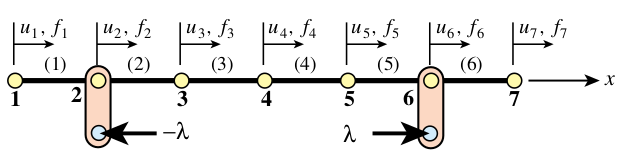
\includegraphics[width=0.70\textwidth]{img/1D_mfc_lagrange_multiplier.png}
    \caption{Physical interpretation of Lagrange multiplier adjuction to enforce
    the MFC $ u_2 = u_6 $}
    \label{fig:1D-MFC-lagrange-multiplier-png}
\end{figure}


\subsection{Physical Interpretation}

As in the case of the penalty function method, the method Lagrange multiplier
can be given a rigorous justification within the framework of variational
calculus. But in the same spirit it will be introduced for the example structure
from a physical standpoint that is particularly illuminating.

Consider again the constraint $ u_2 = u_6 $. Borrowing some ideas from the
penalty method, imagine that nodes 2 and 6 are connected now by
a \textit{rigis} link rather than a flexible one. Thus the constraint is imposed
exactly. But of course the penalty method with an infinite weight would "blow up".

We may remove the link if it is replaced by an appropriate reaction force pair
$ ( -\lambda, +\lambda ) $, as illustrated in Figure
\ref{fig:1D-MFC-lagrange-multiplier-png}. These are called the
\textit{constraint forces}. Incorporating these forces into the original stiffness
equations we get:

\begin{equation}\label{master-stiffness-6-bar-lagrange}
    \begin{bmatrix}
        K_{11} & K_{12} & 0 & 0 & 0 & 0 & 0 \\
        K_{12} & K_{22} & K_{23} & 0 & 0 & 0 & 0 \\
        0 & K_{23} & K_{33} & K_{34} & 0 & 0 & 0 \\
        0 & 0 & K_{34} & K_{44} & K_{45} & 0 & 0 \\
        0 & 0 & 0 & K_{45} & K_{55} & K_{56} & 0 \\
        0 & 0 & 0 & 0 & K_{56} & K_{66} & K_{67} \\
        0 & 0 & 0 & 0 & 0 & K_{67} & K_{77}
    \end{bmatrix}
    \begin{bmatrix}
        u_1 \\
        u_2 \\
        u_3 \\
        u_4 \\
        u_5 \\
        u_6 \\
        u_7
    \end{bmatrix}
    = \begin{bmatrix}
        f_1 \\
        f_2 - \lambda \\
        f_3 \\
        f_4 \\
        f_5 \\
        f_6 + \lambda \\
        f_7
    \end{bmatrix}
\end{equation}

This $ \lambda $ is called \textbf{Lagrange multiplier}. Because $ \lambda $
is an unknown, let us transfer it to the \textbf{LHS} by \textbf{appending} it
to the vector of unknowns:

\begin{equation}
    \begin{bmatrix}
        K_{11} & K_{12} & 0 & 0 & 0 & 0 & 0 & 0 \\
        K_{12} & K_{22} & K_{23} & 0 & 0 & 0 & 0 & 1 \\
        0 & K_{23} & K_{33} & K_{34} & 0 & 0 & 0 & 0 \\
        0 & 0 & K_{34} & K_{44} & K_{45} & 0 & 0 & 0 \\
        0 & 0 & 0 & K_{45} & K_{55} & K_{56} & 0 & 0 \\
        0 & 0 & 0 & 0 & K_{56} & K_{66} & K_{67} & -1 \\
        0 & 0 & 0 & 0 & 0 & K_{67} & K_{77} & 0
    \end{bmatrix}
    \begin{bmatrix}
        u_1 \\
        u_2 \\
        u_3 \\
        u_4 \\
        u_5 \\
        u_6 \\
        u_7 \\
        \lambda
    \end{bmatrix}
    = \begin{bmatrix}
        f_1 \\
        f_2 \\
        f_3 \\
        f_4 \\
        f_5 \\
        f_6 \\
        f_7
    \end{bmatrix}
\end{equation}

But now we have 7 equations for 8 unknowns. To render the system determinate, the
constraint condition $ u_2 - u_6 = 0 $ is appended as eight equation:

\begin{equation}
    \begin{bmatrix}
        K_{11} & K_{12} & 0 & 0 & 0 & 0 & 0 & 0 \\
        K_{12} & K_{22} & K_{23} & 0 & 0 & 0 & 0 & 1 \\
        0 & K_{23} & K_{33} & K_{34} & 0 & 0 & 0 & 0 \\
        0 & 0 & K_{34} & K_{44} & K_{45} & 0 & 0 & 0 \\
        0 & 0 & 0 & K_{45} & K_{55} & K_{56} & 0 & 0 \\
        0 & 0 & 0 & 0 & K_{56} & K_{66} & K_{67} & -1 \\
        0 & 0 & 0 & 0 & 0 & K_{67} & K_{77} & 0 \\
        0 & 1 & 0 & 0 & 0 -1 & 0 & 0
    \end{bmatrix}
    \begin{bmatrix}
        u_1 \\
        u_2 \\
        u_3 \\
        u_4 \\
        u_5 \\
        u_6 \\
        u_7 \\
        \lambda
    \end{bmatrix}
    = \begin{bmatrix}
        f_1 \\
        f_2 \\
        f_3 \\
        f_4 \\
        f_5 \\
        f_6 \\
        f_7 \\
        0
    \end{bmatrix}
\end{equation}

This is called the \textbf{multiplier-augmented} system. Its coefficient matrix,
which is symmetric, is called the \textbf{bordered stiffness matrix}. The
process by which $ \lambda $ is appended to the vector of original unknowns
is called \textbf{adjucation}. Solving this system provides the desired solution
for the DOFs while also characterising the constraint forces through
$ \lambda $.


\subsection{Lagrange Multipliers fro General MFCs}

The general procedure will be stated first as a recipe. Suppose that we want
to solve the example structure subjected to three MFCs:

\begin{equation}
    u_2 - u_6 = 0, \quad 5 u_2 - 8 u_7 = 3, \quad 3 u_3 + u_5 - 4 u_6 = 1
\end{equation}

Adjoin these MFCs as the eighth, nineth, and tenth equations:

\begin{equation}
    \begin{bmatrix}
        K_{11} & K_{12} & 0 & 0 & 0 & 0 & 0 \\
        K_{12} & K_{22} & K_{23} & 0 & 0 & 0 & 0 \\
        0 & K_{23} & K_{33} & K_{34} & 0 & 0 & 0 \\
        0 & 0 & K_{34} & K_{44} & K_{45} & 0 & 0 \\
        0 & 0 & 0 & K_{45} & K_{55} & K_{56} & 0 \\
        0 & 0 & 0 & 0 & K_{56} & K_{66} & K_{67} \\
        0 & 0 & 0 & 0 & 0 & K_{67} & K_{77} \\
        0 & 1 & 0 & 0 & 0 & -1 & 0 \\
        0 & 5 & 0 & 0 & 0 & 0 & -8 \\
        0 & 0 & 3 & 0 & 1 & -4 & 0
    \end{bmatrix}
    \begin{bmatrix}
        u_1 \\
        u_2 \\
        u_3 \\
        u_4 \\
        u_5 \\
        u_6 \\
        u_7
    \end{bmatrix}
    = \begin{bmatrix}
        f_1 \\
        f_2 \\
        f_3 \\
        f_4 \\
        f_5 \\
        f_6 \\
        f_7 \\
        0 \\
        3 \\
        1
    \end{bmatrix}
\end{equation}

Three Lagrange multipliers: $ \lambda_1, \lambda_2 $ and $ \lambda_3 $ are
required to care of three MFCs. Adjoin those unknowns to the nodal displacement
vector. Symmetrize the coefficient matrix by appending 3 columns that are the
transpose of the 3 last rows and filling the bottom righ-hand corner with
a $ 3 \times 3 $ zero matrix:

\begin{equation}
    \begin{bmatrix}
        K_{11} & K_{12} & 0 & 0 & 0 & 0 & 0 & 0 & 0 & 0 \\
        K_{12} & K_{22} & K_{23} & 0 & 0 & 0 & 0 & 1 & 5 & 0 \\
        0 & K_{23} & K_{33} & K_{34} & 0 & 0 & 0 & 0 & 0 & 3 \\
        0 & 0 & K_{34} & K_{44} & K_{45} & 0 & 0 & 0 & 0 & 0 \\
        0 & 0 & 0 & K_{45} & K_{55} & K_{56} & 0 & 0 & 0 & 1 \\
        0 & 0 & 0 & 0 & K_{56} & K_{66} & K_{67} & -1 & 0 & -4 \\
        0 & 0 & 0 & 0 & 0 & K_{67} & K_{77} & 0 & -8 & 0 \\
        0 & 1 & 0 & 0 & 0 & -1 & 0 & 0 & 0 & 0 \\
        0 & 5 & 0 & 0 & 0 & 0 & -8 & 0 & 0 & 0 \\
        0 & 0 & 3 & 0 & 1 & -4 & 0 & 0 & 0 & 0
    \end{bmatrix}
    \begin{bmatrix}
        u_1 \\
        u_2 \\
        u_3 \\
        u_4 \\
        u_5 \\
        u_6 \\
        u_7 \\
        \lambda_1 \\
        \lambda_2 \\
        \lambda_3
    \end{bmatrix}
    = \begin{bmatrix}
        f_1 \\
        f_2 \\
        f_3 \\
        f_4 \\
        f_5 \\
        f_6 \\
        f_7 \\
        0 \\
        3 \\
        1
    \end{bmatrix}
\end{equation}


\subsection{The Theory Behind}

The recipe illustrated above comes from a well known technique of variational
calculus. Using the matrix notation introduced, compactly denote the set of
$ m $ MFCs by $ \m{A} \m{u} = \m{b} $, where $ \m{A} $ is
$ m \times n $. The potential energy of the unconstrained finite element model is
$ \prod = \frac{1}{2} \m{u}^T \m{K} \m{u} - \m{u}^T \m{f} $.
To impose the constraint, adjoin $ m $ Lagrange multipliers collected in vector
$ \lambda $ and form the Lagrangian

\begin{equation}
    \lagr(\m{u}, \M{\lambda}) = \prod + \M{\lambda}
    \left( \m{A} \m{u} - \m{b}\right)
    = \frac{1}{2} \m{u}^T \m{K} \m{u} - \m{u}^T \m{f} + \M{\lambda}^T
    \left( \m{A} \m{u} - \m{b}\right)
\end{equation}

Extremizing $ \lagr $ with respect to $ \m{u} $ and $ \M{\lambda} $ yields
the multiplier-augmented form

\begin{equation}\label{mfc-multiplier-augmented-form}
    \begin{bmatrix}
        \m{K} & \m{A}^T \\
        \m{A} & \m{0}
    \end{bmatrix}
    \begin{bmatrix}
        \m{u} \\
        \M{\lambda}
    \end{bmatrix}
    = \begin{bmatrix}
        \m{f} \\
        \m{b}
    \end{bmatrix}
\end{equation}

The master stiffness matrix $ \m{K} $ is said to be \textbf{bordered} with
$ \m{A} $ and $ \m{A}^T $. Solving this system provides $ \m{u} $ and $ \M{\lambda} $.
The latter can be interpreted as forces of constraint in the following sense:
a removed constraint can be replaced by a system of forces characterised by
$ \M{\lambda} $ multiplied by the constraint coefficients. More precisely,
the constraint forces are $ -\m{A}^T \M{\lambda} $.


\subsection{Assesment of the Lagrange Multiplier Method}

In contrast to the penalty method, the method of Lagrange multipliers has the
advantage of being exact (aside from computational errors due to finite
precision arithmetic). It provides directly the constraint forces, which are of
interest in many applications. It does not require guesses as regards to weights.
As the penalty method, it can be extended without difficulty to nonlinear constraints.

It is not free of disadvantages. It introduces additional unknowns, requiring
expansion of the original stiffness method, and more complicated storage allocation
procedures. It renders the augmented stiffness matrix indefinite, na effect that
may cause grief with some linear equation solving methods that rely on positive
definiteness. Finally, as the master-slave method, it is sensitive to the degree
of linear independence of the constraints: if the constraint $ u_2 = u_6 $ is
specified twice, the bordered stiffness is obviously singular.

On the whole this method appears to be the most elegant one for a general-purpose
finite element program that is supposed to work as a "black box" by minimizing
guesses and choices from its users. Its implementation, however, is not simple.
Special care must be excercised to detect singularities due to constraint
dependency and to account for the effect of loss of positive definiteness of the
bordered stiffness on equation solver.


\subsection{The Augmented Lagrangian Method}

The general matrix of the penalty function and Lagrangian multiplier methods are
given by expressions \eqref{mfc-augmented-potential-energy} and
\eqref{mfc-multiplier-augmented-form}, respectively. A useful connection
between these methods can be established as follows.

Because the lowe diagonal block of the bordered stiffness matrix in
\eqref{mfc-multiplier-augmented-form} is null, it is not possible to directly
eliminate $ \M{\lambda} $. To make this possible, replace this block by
$ \epsilon \m{S}^{-1} $, where $ \m{S} $ is a constraint-scaling diagonal matrix
of appropriate order and $ \epsilon $ is a small number. The reciprocal of
$ \epsilon $ is a large number called $ w = 1 / \epsilon $. To maintain
exactness of the second equation, $ \epsilon \m{S}^{-1} \M{\lambda} $ is added
to the RHS:

\begin{equation}\label{mfc-lagrangian}
    \begin{bmatrix}
        \m{K} & \m{A}^T \\
        \m{A} & \epsilon \m{S}^{-1}
    \end{bmatrix}
    \begin{bmatrix}
        \m{u} \\
        \M{\lambda}
    \end{bmatrix}
    = \begin{bmatrix}
        \m{f} \\
        \epsilon \m{S}^{-1} \M{\lambda}^P
    \end{bmatrix}
\end{equation}

Here superscript $ P $ (for "predicted" value) is attached to the $ \M{\lambda} $
on the RHS as a "tracer". We can now formally solve for $ \M{\lambda} $
and subsequently for $ \m{u} $. The results may be presented as:

\begin{eqarray}\label{mfc-lagrange-augmented-decomposed}
    \left( \m{K} + w \m{A}^T \m{S} \m{A} \right) \m{u}
    &= \m{f} + w \m{A}^T \m{S} \m{b} - \m{A}^T \M{\lambda}^P \\
    \M{\lambda} &= \M{\lambda}^P + w \m{S} \left(\m{b} - \m{A} \m{u} \right)
\end{eqarray}

Setting $ \M{\lambda}^P  = \m{0} $ in the first matrix equation yields:

\begin{equation}
    \left( \m{K} + w \m{A}^T \m{S} \m{A} \right) \m{u}
    = \m{f} + w \m{A}^T \m{S} \m{b}
\end{equation}

on taking $ \m{W} = w \m{S} $, the general matrix equation
\eqref{mfc-augmented-potential-energy} of the penalty method is recovered.

This relation suggests the construction of \textit{iterative procedures}
in which one tries to \textit{improve the accuracy of the penalty function}
\textit{while} $ w $ \textit{is kept constant}. This strategy circumvents the
aforementioned ill-conditioning problems when the weight $ w $ is gradually
increased. One such method is easily constructed by inspecting
\eqref{mfc-lagrange-augmented-decomposed}. Using superscript $ k $ as an
iteration index and keeping $ w $ fixed, solve equations
\eqref{mfc-lagrange-augmented-decomposed} in tandem as follows:

\begin{eqarray}\label{mfc-lagrange-augmented-iteration}
    \left( \m{K} + \m{A}^T \m{W} \m{A} \right) \m{u}^k
    &= \m{f} + \m{A}^T \m{W} \m{b} - \m{A}^T \M{\lambda}^k \\
    \M{\lambda}^{k+1} &= \M{\lambda}^k + \m{W} \left(\m{b} - \m{A} \m{u}^k \right)
\end{eqarray}

for $ k = 0, 1, \dots $, beginning with $ \M{\lambda}^0 = 0 $. Then $ \m{u}^0 $
is the penalty solution. If the process converges one recovers the exact Lagrangian
solution without having to solve the Lagrangian system \eqref{mfc-lagrangian}
directly.

The family of iterative procedures that may be precipitated from
\eqref{mfc-lagrange-augmented-decomposed} collectively pertains to the class of
\textit{augmented Lagrangian methods}.


\section{Summary}

The treatment of linear MFCs in finite element systems can be carried out by
several methods. Three of these: \textbf{master-slave elimination},
\textbf{penalty augmentation} and \textbf{Lagrange multiplier} adjunction
have been discussed.

It is emphasised that no method is uniformly satisfactory in terms of generality,
robustness, numerical behavior and simplicity of implementation.

For a general purpose program that tries to attain "black box" behavior
(that is minimal decisions on the part of users) the Lagrange multipliers has
the edge. This edge is unfortunately blunted by a fairly complex computer
implementation and by the loss of positive definiteness in the bordered stiffness
matrix.


